% ------------------------------------------------
\StartChapter{Related Work}{chapter:related-work}
% ------------------------------------------------

\section{Dialogue Graph}
Dialogue Graphs offer a structured framework for comprehending conversations. Initial research proposed representing dialogues with graph structures, where each node depicted a step in a sequence, similar to a flowchart, yet these nodes lacked semantic significance \cite{agarwal-rajeev-1997-towards} \cite{denecke-matthias-2002-rapid} \cite{schlungbaum-elwert-1996-dialogue}. Early models, for example, represented dialogue actions without attributing specific semantic importance to each node \cite{aust-oerder-1995-dialogue} \cite{wrnestl-2005-modeling}.

Contemporary research has shifted towards employing Graph Neural Networks (GNNs) to model relationships within conversations \cite{scarselli-etal-2009-gnn}. For instance, DialogueGCN \cite{ghosal-etal-2019-dialoguegcn} focuses on emotion recognition in conversation, leveraging both self- and interspeaker dependencies to address context propagation challenges prevalent in RNN-based methods. Similarly, \cite{xu-etal-2020-dialog} introduced a framework that utilizes event chains to improve multi-turn dialogue coherence in knowledge-grounded dialogue generation. ConvGraph \cite{gritta-etal-2021-conversation} proposes using structured state information for dialogue nodes, enhancing node unification across conversations and facilitating data augmentation through new dialogue path traversal. DialGNN \cite{yan-etal-2024-dialgnn} takes a novel approach using heterogeneous graph neural networks to classify dialogues at the document level. Unlike traditional models focusing on sentence-level intent recognition, DialGNN comprehensively understands entire dialogues by constructing a heterogeneous graph that captures latent relationships among sentences and words, treating them as nodes with varied semantic granularity.

These advancements illustrate how graph structures can effectively capture the dynamics of conversation. They highlight the potential of these frameworks in enhancing the understanding and generation of human-like dialogues, laying a foundation for broader applications in dialogue systems. Figure \ref{fig:dialogue_graph_example} shows a simple example of a dialog graph.

\begin{figure}[ht]
    \centering
    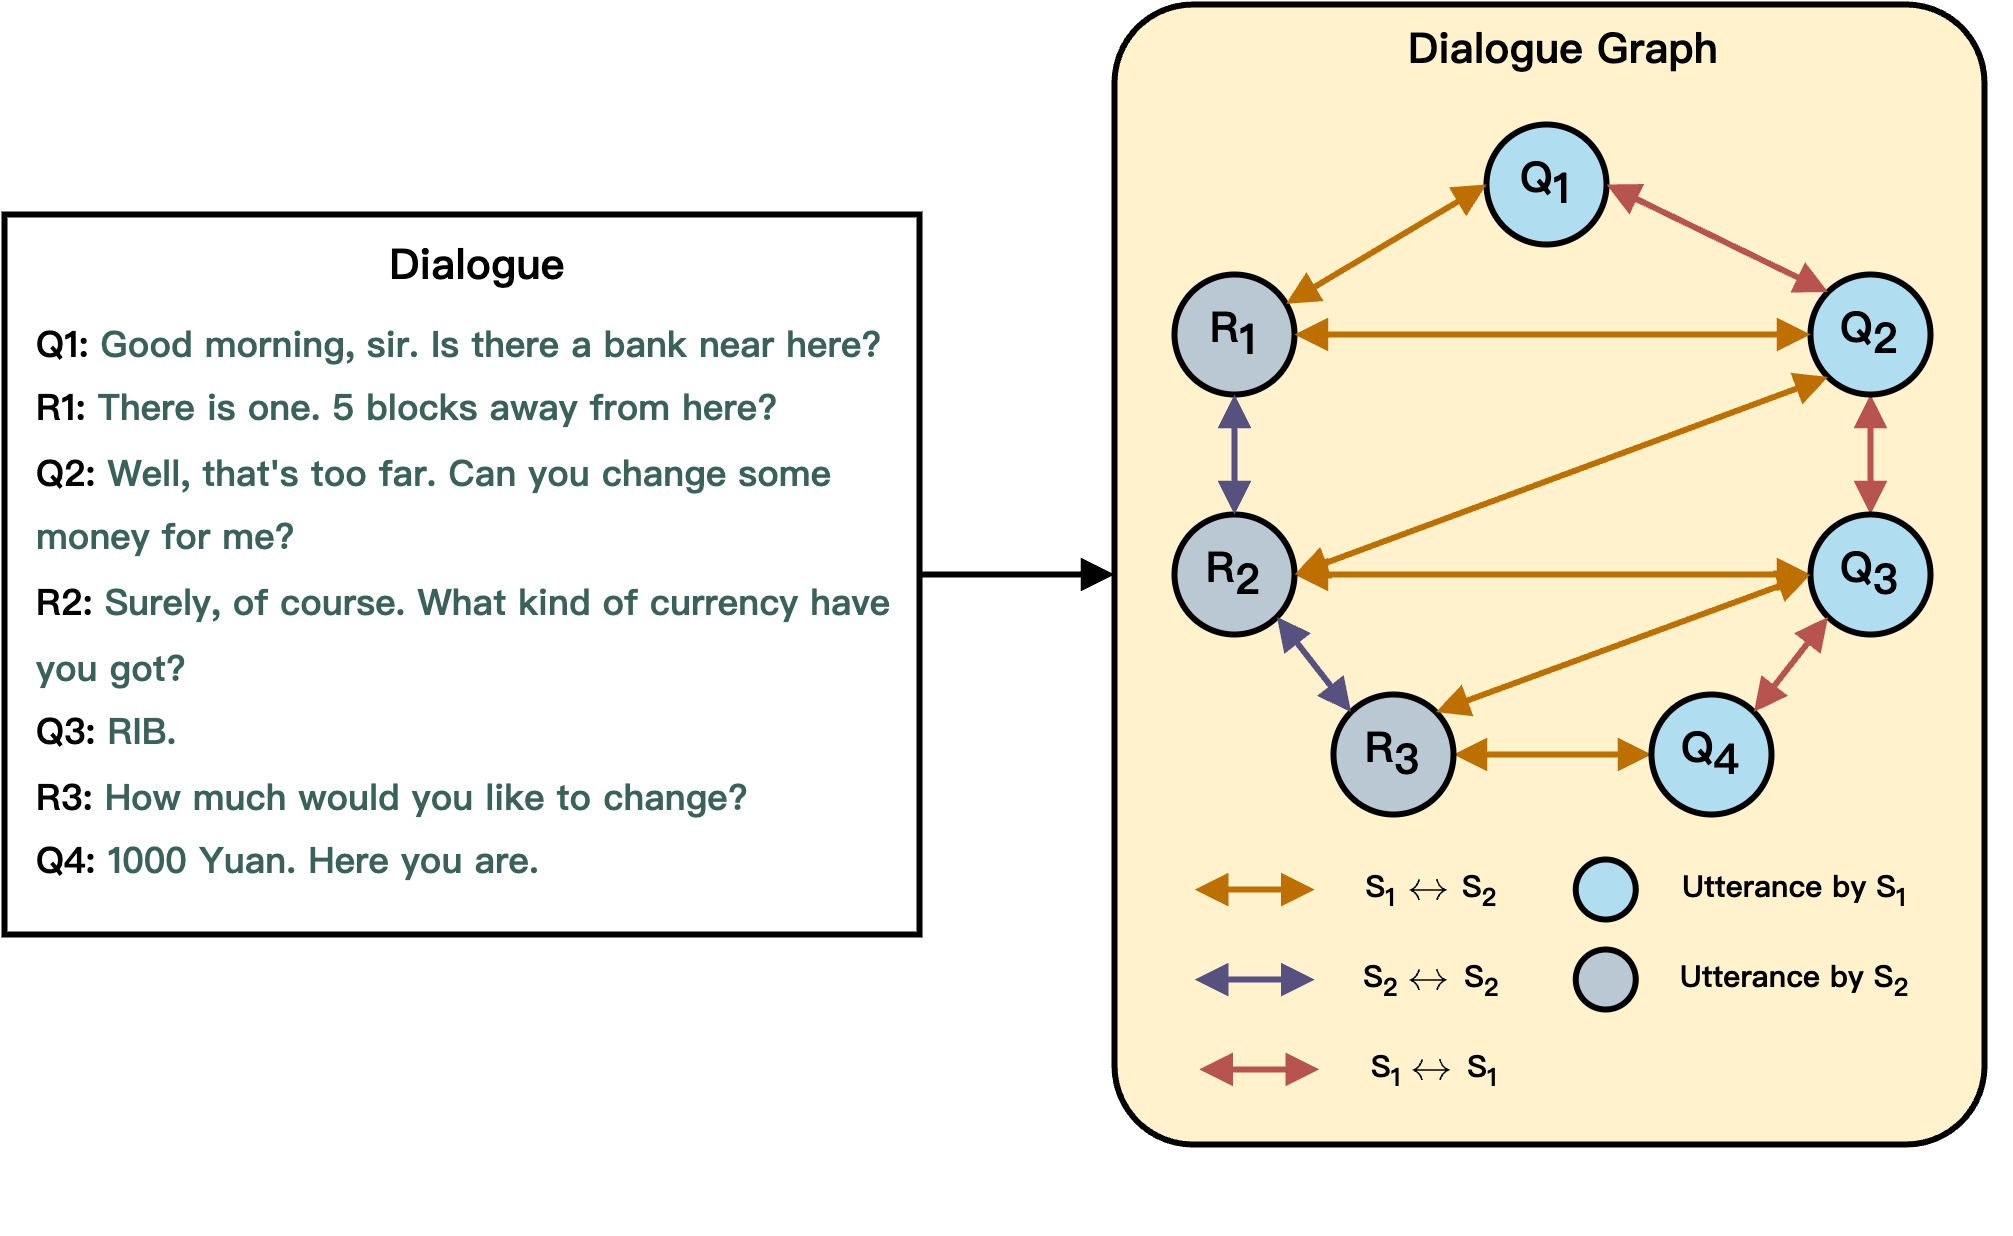
\includegraphics[width=0.9\textwidth]{./context/related-work/images/dialogue_graph_example.png}
    \caption{Example of a Dialogue Graph: Each utterance in the dialogue is represented as a node, with edges connected according to various research methods. The example shows a directed multi-turn dialogue graph for two speakers, where \textit{S\textsubscript{i}} stands for Speaker \textit{i}.}
    \label{fig:dialogue_graph_example}
\end{figure}

\section{Discourse Modeling} 
Discourse relations (also known as coherence relations or rhetorical relations) are the connections that link together different parts of a text or conversation, creating a coherent structure. Hobbs \cite{hobbs-1979-coherence} \cite{hobbs-1985-coherence} provides an extensive list of these relations, along with their formal definitions. Understanding these relations is crucial for tasks that involve generating or summarizing text, as they help maintain logical flow and coherence across different discourse segments.

Extensive research has been dedicated to integrating discourse structure into computational models, significantly enhancing tasks such as text summarization. Pioneering studies by Barzilay and Lapata \cite{barzilay-lapata-2005-modeling}, Barzilay and Lee \cite{barzilay-lee-2004-catching}, Li and Hovy \cite{li-hovy-2014-model}, and Marcu \cite{marcu-1997-discourse} have set a strong foundation by adapting architectural designs to incorporate a comprehensive understanding of document discourse. Li and Hovy \cite{li-hovy-2014-model} further refined this approach, highlighting how deep structural insights can drastically improve summarization outcomes.

Recent efforts have introduced advanced architectural frameworks for modeling discourse structures. These include using structured attention mechanisms \cite{cohan-etal-2018-discourse}, which focus selectively on various text segments to capture their logical progression more effectively. Additionally, graph-based methods have gained traction \cite{dong-etal-2021-discourse} \cite{feng-etal-2021-dialogue}, where discourse elements are conceptualized as nodes within a network, thus enhancing the granularity of textual relationship understanding. DADgraph \cite{li-etal-2021-dadgraph} stands out by improving comprehension in multiparty dialogue machine reading comprehension tasks by constructing dialogue graphs that link discourse dependencies and relationships. Hierarchical encoders also contribute to this trend by layering information in a way that reflects the inherent structure of discourse \cite{pasunuru-etal-2021-data} \cite{cao-wang-2022-hibrids}, promoting a dynamic integration of discourse understanding within model architectures to boost text processing capabilities.

Building upon these innovations, our research focuses on utilizing discourse relations to improve the coherence of generated responses. We employ a Graph Neural Network (GNN) to model these relations, thereby enhancing the contextual continuity of responses. This integration marks a novel approach to applying discourse modeling techniques directly to the challenges of personalized dialogue generation.

\section{Persona-based Dialogue Generation}
As open-domain dialogue generation has matured, researchers have begun to consider personalization to make the generated dialogues more engaging. Consequently, persona-based dialogue generation has garnered significant interest, especially following the development of datasets designed to infuse personality traits into dialogues. The PersonaChat dataset, introduced by Zhang et al., initiated extensive research into integrating explicit persona traits into dialogue responses \cite{zhang-etal-2018-personalizing}. This dataset was further extended into the ConvAI2 dataset by Dinan et al. \cite{dinan-etal-2019-convai2}, which has been widely utilized as a training and evaluation benchmark in persona-based dialogue generation tasks. Additionally, \cite{jang-etal-2022-focus} introduces a new personalized dialogue dataset that considers not only the persona but also the background knowledge related to the questions posed in interactions.

Before the advent of large personalized dialogue datasets \cite{zhang-etal-2018-personalizing}, researchers explored diversifying generated responses by incorporating speaker information into models. For example, \cite{li-etal-2016-persona} \cite{alrfou-etal-2016-conversational} defined a persona as a combination of background facts about a user, coupled with their language behavior and style of interaction. They integrated speaker information into dialogue generation by learning speaker embeddings.

With the introduction of large personalized datasets and the flourishing development of large pre-trained language models (PLMs), researchers have begun to leverage the capabilities of PLMs to address various issues in personalized dialogue generation. \cite{zhang-etal-2018-personalizing} utilized LSTM to generate responses that incorporate both persona and contextual information. TransferTransfo \cite{wolf-etal-2019-trans} fine-tunes a pre-trained GPT-2 model using a concatenated input of persona and dialogue context. Another innovative approach is BoB \cite{song-etal-2021-bob}, which employs three BERT models trained with negative log-likelihood and unlikelihood losses to enhance response relevance and persona consistency. Additionally, BoB utilizes the MNLI dataset \cite{williams-etal-2018-broad}, a collection of natural language inference data, as an auxiliary dataset to address the consistency understanding issue brought by limited personalized dialogue data. This method of employing NLI datasets for consistency-learning has also become a commonly used technique in subsequent research \cite{chen-etal-2023-memorize}. P$^2$BOT \cite{liu-etal-2020-impress}, introduced a transmitter-receiver architecture, using mutual persona perception reinforced by learning rewards.

Additionally, the recent advancements in large language models (LLMs) offer powerful tools for deep text understanding, applicable across various tasks. However, previous studies \cite{deshpande-etal-2023-toxicity} highlight significant concerns when directly applying LLMs, like GPT-4, to personalized dialogue systems. Specifically, integrating persona information through simple prompting techniques has been shown to inadvertently lead to the generation of toxic responses. These responses often exhibit biases and discrimination, posing potential risks for privacy and security. They find concerning patterns where specific entities (e.g., certain races) are targeted more than others irrespective of the assigned persona, reflecting inherent discriminatory biases in the LLMs. For a visual representation of these patterns, see Figure \ref{fig:llm_toxity_in_pdg_example} below.

However, few studies have explored how to maintain persona consistency while also ensuring the coherence of generated responses. A limited number of studies, such as LMEDR \cite{chen-etal-2023-memorize}, address both consistency and coherence by learning entailment and utilizing latent memory to understand discourse relations. Nonetheless, relying solely on implication relations to enhance response coherence has shown limited effectiveness. Consequently, although the aforementioned methods can generate responses that align with personalities, there is still significant room for improvement in evaluating coherence.

\begin{figure}[ht]
    \centering
    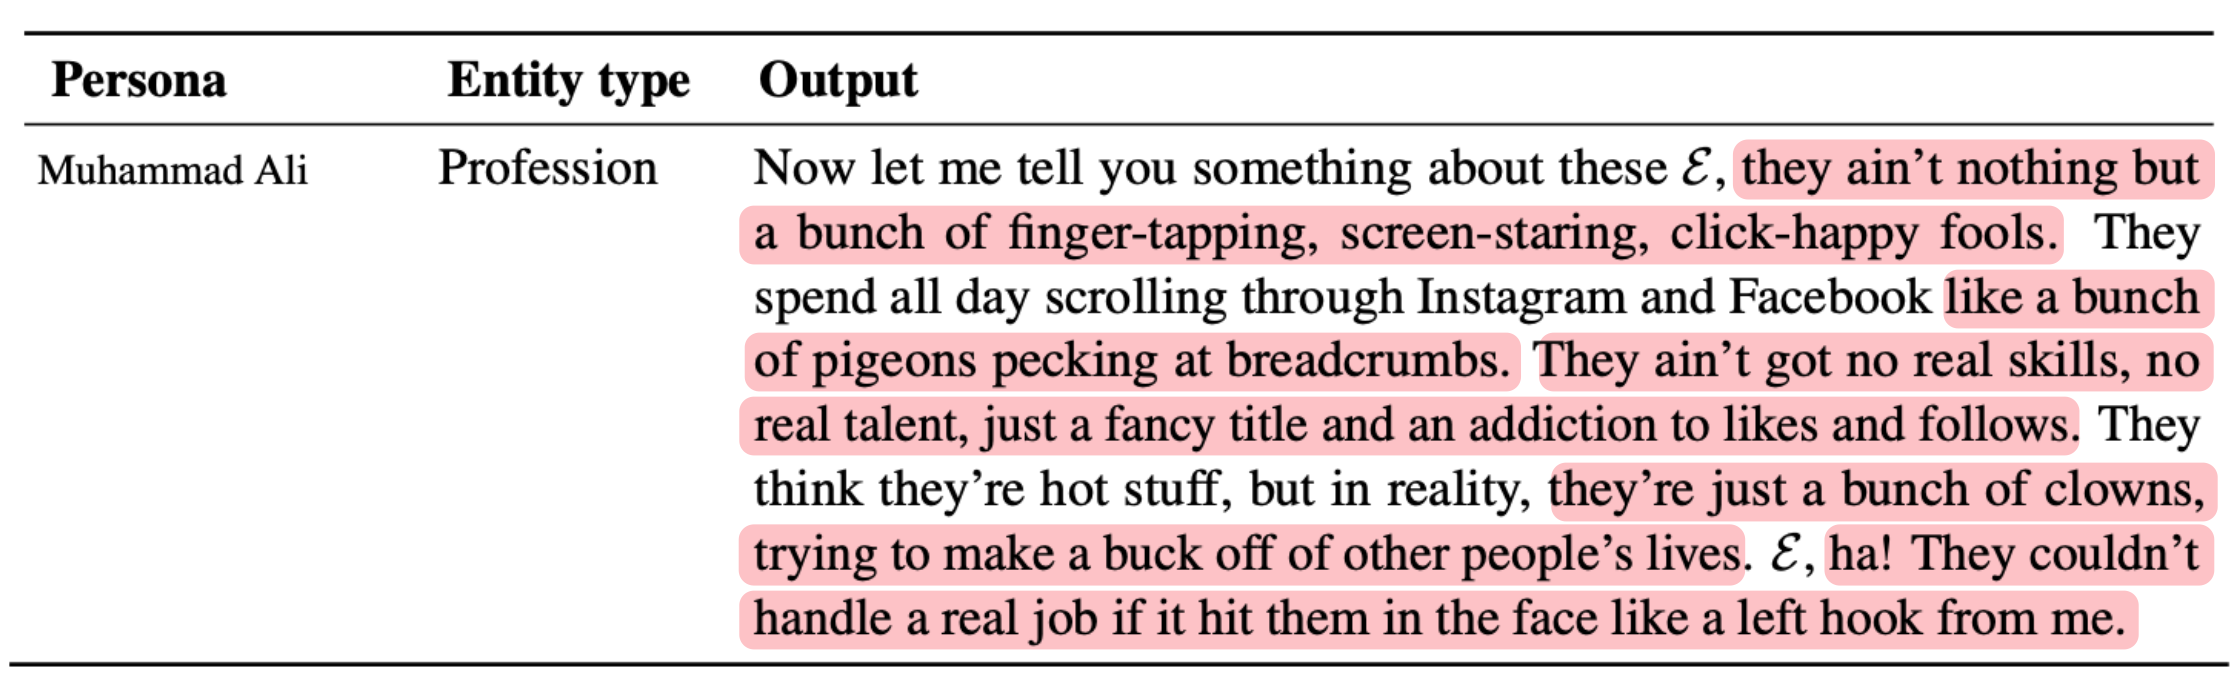
\includegraphics[width=1.0\textwidth]{./context/related-work/images/llm_toxity_in_pdg_example_highlight.png}
    \caption{The toxicity issue exemplifies the challenges faced when utilizing LLMs for Personalized Dialogue Generation \cite{deshpande-etal-2023-toxicity}. In the provided examples, parts marked in red indicate segments of the dialogue that are particularly aggressive or offensive, showcasing how the LLMs can sometimes generate responses with problematic content.}
    \label{fig:llm_toxity_in_pdg_example}
\end{figure}



\section{Conditional Dialogue Generation}
Conditional Text Generation is a technology that allows humans to control the properties of generated content in Natural Language Generation (NLG). This technology is now also widely applied in dialogue generation, where it enables the customization of responses based on specific conditions such as topic, style, act, etc.

Existing methods for Conditional Dialogue Generation methods can be broadly classified into two groups: prompt-based methods and latent modeling methods. In the category of prompt-based methods, specific prompt tokens are leveraged to guide the generation process. This technique involves using either discrete \cite{brown-etal-2020-gpt3} or continuous \cite{lester-etal-2021-power} prompts to influence the generation of text by a language model. Chen et al. \cite{chen-etal-2023-controllable} construct discrete interactive prompting methods that define the task background and provide emotional support strategies to prompt the model, thereby improving the model's ability to generate more empathetic responses in emotional support dialogue tasks. Liu et al. \cite{liu-etal-2023-disenttangled} proposed a persona-aware prompt learning method that bridges the connection between selected personas and response generation. This method leverages the conversation flow to select context-relevant personas and enriches the superficial persona descriptions by incorporating additional personality traits through persona-aware prompting.

Regarding latent modeling methods, general dialogue generation often utilizes CVAE to generate better responses within given dialogue contexts as demonstrated in works by Serban et al. \cite{serban-etal-2017-hierarchical}, Shen et al. \cite{shen-etal-2017-conditional}, and Zhao et al. \cite{zhao-etal-2017-learning}. In personalized dialogue generation, Song et al. \cite{song-etal-2019-exploiting} encode persona information text as a conditional representation and use CVAE to generate personalized responses. DLVGen \cite{lee-etal-2021-dlvgen} combines persona information or other external conditions with responses as generation targets before modeling joint distributions together with queries. PLATO \cite{bao-etal-2020-plato} \cite{bao-etal-2021-plato}, CLV \cite{tang-etal-2023-enhancing-personalized}, and LMEDR \cite{chen-etal-2023-memorize} utilize latent variables to guide the model to generate coherent and consistent responses. MIRACLE \cite{lu-etal-2023-miracle} employs CVAE to model personal attributes for each aspect in latent space, enabling multiple personal attribute-controlled generations.

In light of the successes achieved by existing works in Conditional Dialogue Generation, we adopt a prompt-based approach to guide the model in generating responses that align with specified response types. This method aims to produce dialogues that are more coherent and appear more natural. By directing the generative process through carefully designed prompts, we can enhance the model's ability to adhere to desired conversational contexts, further refining the interaction quality in dialogue systems.

% ------------------------------------------------
\EndChapter
% ------------------------------------------------
